\documentclass[tikz,border=8pt]{standalone}
\usepackage{tikz}
\usepackage{pgfplots}
\usepackage{amsmath, amssymb}

\pgfplotsset{compat=1.18}

\begin{document}

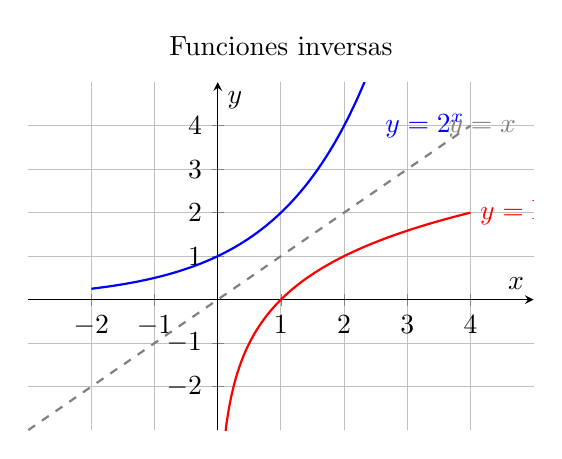
\begin{tikzpicture}[scale=1.0]

  \begin{axis}[
    axis lines = middle,
    xlabel = {$x$},
    ylabel = {$y$},
    title = {Funciones inversas},
    xmin = -3, xmax = 5,
    ymin = -3, ymax = 5,
    xtick = {-2,-1,0,1,2,3,4},
    ytick = {-2,-1,0,1,2,3,4},
    grid = major,
    width = 8cm,
    height = 6cm,
  ]

    % Función exponencial y = 2^x
    \addplot[blue, thick, domain=-2:2.5, samples=100] {2^x};
    \node[blue, right] at (axis cs:2.5, 4) {$y = 2^x$};

    % Función logarítmica y = log2(x)
    \addplot[red, thick, domain=0.1:4, samples=100] {ln(x)/ln(2)};
    \node[red, right] at (axis cs:4, 2) {$y = \log_2(x)$};

    % Recta identidad y = x (eje de simetría)
    \addplot[gray, dashed, thick, domain=-3:4] {x};
    \node[gray, above right] at (axis cs:3.5, 3.5) {$y = x$};

  \end{axis}

\end{tikzpicture}

\end{document}
